\section{Learning Objectives}

After completing this chapter, readers will be able to:
\begin{itemize}
    \item Understand when distributed training is necessary and beneficial
    \item Distinguish between data parallelism and model parallelism strategies
    \item Implement distributed training using PyTorch DistributedDataParallel
    \item Use Horovod for framework-agnostic distributed training
    \item Apply Ray for scalable distributed training workflows
    \item Design gradient synchronization strategies (synchronous vs asynchronous)
    \item Implement fault tolerance mechanisms for long-running training jobs
    \item Optimize communication overhead in distributed training
    \item Benchmark and profile distributed training performance
    \item Allocate and schedule resources efficiently across clusters
\end{itemize}

\section{Introduction: The Scale Challenge}

Modern deep learning models have grown exponentially in size and complexity. GPT-3 has 175 billion parameters, while models like PaLM reach 540 billion parameters. Training such models on a single GPU is impossible—distributed training is essential.

\subsection{When to Use Distributed Training}

Distributed training becomes necessary when:

\begin{itemize}
    \item \textbf{Model Too Large:} Model parameters exceed single GPU memory (>24GB)
    \item \textbf{Dataset Too Large:} Training data doesn't fit in memory or takes days/weeks
    \item \textbf{Time Constraints:} Single-GPU training exceeds acceptable timeframes
    \item \textbf{Batch Size Requirements:} Larger effective batch sizes needed for convergence
    \item \textbf{Hyperparameter Search:} Parallel exploration of hyperparameter space
\end{itemize}

\begin{example}[Cost-Benefit Analysis]
Training a large vision model:
\begin{itemize}
    \item \textbf{Single V100 GPU:} 14 days, \$672 (AWS p3.2xlarge)
    \item \textbf{8x V100 GPUs:} 2 days, \$768 (AWS p3.16xlarge)
    \item \textbf{16x V100 GPUs:} 1 day, \$768 (2x p3.16xlarge)
\end{itemize}

The 8-GPU setup offers the best balance: 7x speedup for only 14\% cost increase.
\end{example}

\subsection{Distributed Training Challenges}

Distributed training introduces complexity:

\begin{enumerate}
    \item \textbf{Communication Overhead:} Synchronizing gradients across workers
    \item \textbf{Load Balancing:} Ensuring equal workload distribution
    \item \textbf{Fault Tolerance:} Handling worker failures gracefully
    \item \textbf{Scaling Efficiency:} Diminishing returns as worker count increases
    \item \textbf{Debugging Complexity:} Harder to diagnose issues across multiple processes
    \item \textbf{Infrastructure Management:} Coordinating distributed resources
\end{enumerate}

\section{Parallelism Strategies}

There are two fundamental approaches to distributed training: data parallelism and model parallelism.

\subsection{Data Parallelism}

Data parallelism replicates the model across multiple devices, with each device processing different data batches.

\subsubsection{How Data Parallelism Works}

\begin{figure}[h]
\centering
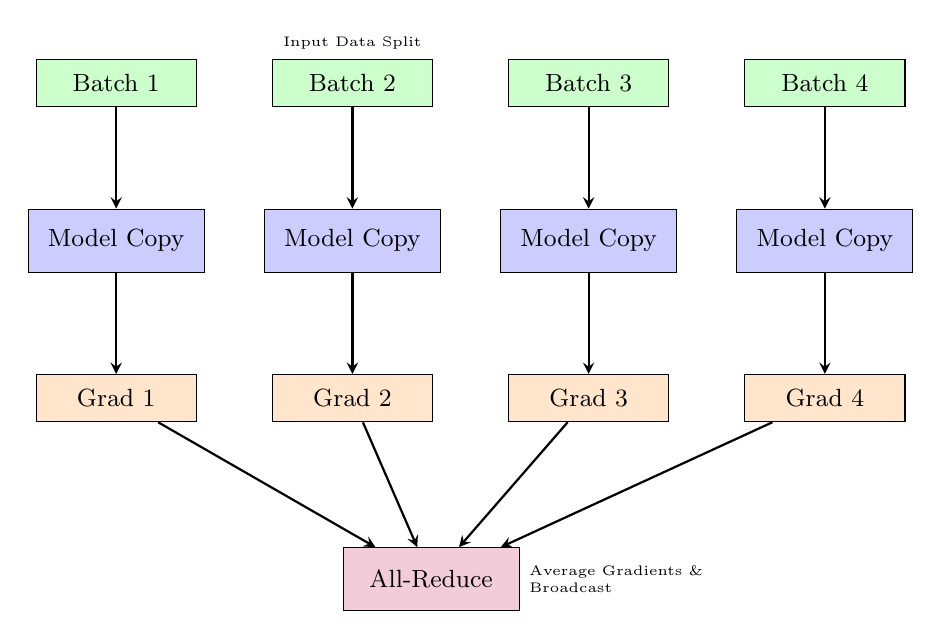
\begin{tikzpicture}[
    node distance=1.5cm,
    box/.style={rectangle, draw, fill=blue!20, text width=2cm, text centered, minimum height=0.8cm, font=\small},
    data/.style={rectangle, draw, fill=green!20, text width=1.8cm, text centered, minimum height=0.6cm, font=\small},
    arrow/.style={->, >=stealth, thick}
]
    % Data batches
    \node[data] (data1) {Batch 1};
    \node[data, right of=data1, xshift=1.5cm] (data2) {Batch 2};
    \node[data, right of=data2, xshift=1.5cm] (data3) {Batch 3};
    \node[data, right of=data3, xshift=1.5cm] (data4) {Batch 4};

    % Model replicas
    \node[box, below of=data1, yshift=-0.5cm] (model1) {Model Copy};
    \node[box, below of=data2, yshift=-0.5cm] (model2) {Model Copy};
    \node[box, below of=data3, yshift=-0.5cm] (model3) {Model Copy};
    \node[box, below of=data4, yshift=-0.5cm] (model4) {Model Copy};

    % Gradients
    \node[data, below of=model1, yshift=-0.5cm, fill=orange!20] (grad1) {Grad 1};
    \node[data, below of=model2, yshift=-0.5cm, fill=orange!20] (grad2) {Grad 2};
    \node[data, below of=model3, yshift=-0.5cm, fill=orange!20] (grad3) {Grad 3};
    \node[data, below of=model4, yshift=-0.5cm, fill=orange!20] (grad4) {Grad 4};

    % All-reduce
    \node[box, below of=grad2, xshift=1cm, yshift=-0.8cm, fill=purple!20] (allreduce) {All-Reduce};

    % Arrows
    \draw[arrow] (data1) -- (model1);
    \draw[arrow] (data2) -- (model2);
    \draw[arrow] (data3) -- (model3);
    \draw[arrow] (data4) -- (model4);

    \draw[arrow] (model1) -- (grad1);
    \draw[arrow] (model2) -- (grad2);
    \draw[arrow] (model3) -- (grad3);
    \draw[arrow] (model4) -- (grad4);

    \draw[arrow] (grad1) -- (allreduce);
    \draw[arrow] (grad2) -- (allreduce);
    \draw[arrow] (grad3) -- (allreduce);
    \draw[arrow] (grad4) -- (allreduce);

    % Labels
    \node[above, font=\tiny] at (data2.north) {Input Data Split};
    \node[right, font=\tiny, text width=2.5cm] at (allreduce.east) {Average Gradients \& Broadcast};
\end{tikzpicture}
\caption{Data Parallelism Architecture}
\label{fig:data_parallelism}
\end{figure}

\textbf{Advantages:}
\begin{itemize}
    \item Simple to implement
    \item Works with most models
    \item Scales well up to 100s of GPUs
    \item Minimal code changes
\end{itemize}

\textbf{Disadvantages:}
\begin{itemize}
    \item Each device must hold full model
    \item Communication overhead grows with model size
    \item Limited by single-device memory
\end{itemize}

\subsection{Model Parallelism}

Model parallelism splits the model across devices, with each device computing a portion of the model.

\subsubsection{Pipeline Parallelism}

Pipeline parallelism divides the model into sequential stages:

\begin{figure}[h]
\centering
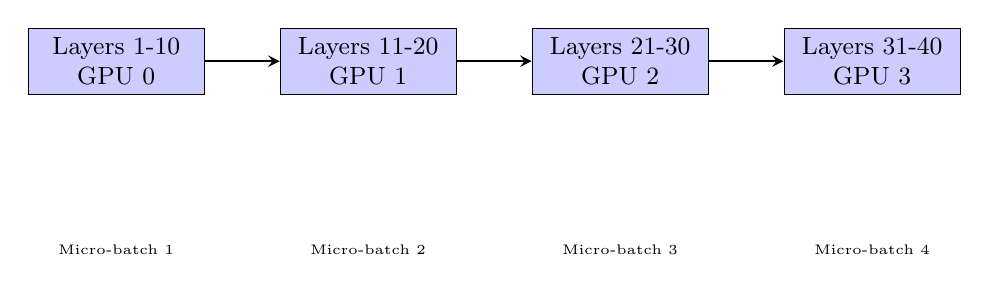
\begin{tikzpicture}[
    node distance=1.2cm,
    box/.style={rectangle, draw, fill=blue!20, text width=2cm, text centered, minimum height=0.8cm, font=\small},
    arrow/.style={->, >=stealth, thick}
]
    % Stages
    \node[box] (stage1) {Layers 1-10\\GPU 0};
    \node[box, right of=stage1, xshift=2cm] (stage2) {Layers 11-20\\GPU 1};
    \node[box, right of=stage2, xshift=2cm] (stage3) {Layers 21-30\\GPU 2};
    \node[box, right of=stage3, xshift=2cm] (stage4) {Layers 31-40\\GPU 3};

    % Arrows
    \draw[arrow] (stage1) -- (stage2);
    \draw[arrow] (stage2) -- (stage3);
    \draw[arrow] (stage3) -- (stage4);

    % Micro-batches
    \node[below of=stage1, yshift=-1.2cm, font=\tiny] (mb1) {Micro-batch 1};
    \node[below of=stage2, yshift=-1.2cm, font=\tiny] (mb2) {Micro-batch 2};
    \node[below of=stage3, yshift=-1.2cm, font=\tiny] (mb3) {Micro-batch 3};
    \node[below of=stage4, yshift=-1.2cm, font=\tiny] (mb4) {Micro-batch 4};
\end{tikzpicture}
\caption{Pipeline Parallelism with Micro-batching}
\label{fig:pipeline_parallelism}
\end{figure}

\textbf{Advantages:}
\begin{itemize}
    \item Enables training of very large models
    \item Reduces per-device memory requirements
    \item Can combine with data parallelism
\end{itemize}

\textbf{Disadvantages:}
\begin{itemize}
    \item Pipeline bubbles reduce efficiency
    \item Complex to implement correctly
    \item Requires careful load balancing
\end{itemize}

\subsubsection{Tensor Parallelism}

Tensor parallelism splits individual layers across devices:

\begin{lstlisting}[style=python, caption=Tensor Parallelism Conceptual Example]
# Standard linear layer: Y = XW + b
# X: [batch_size, input_dim]
# W: [input_dim, output_dim]

# Tensor parallelism splits W column-wise across GPUs:
# GPU 0: W0 = W[:, :output_dim//2]
# GPU 1: W1 = W[:, output_dim//2:]

# Each GPU computes partial output:
# GPU 0: Y0 = XW0
# GPU 1: Y1 = XW1

# Concatenate results: Y = [Y0, Y1]
\end{lstlisting}

\subsection{Hybrid Parallelism}

Production systems often combine strategies:

\begin{table}[h]
\centering
\caption{Parallelism Strategy Comparison}
\label{tab:parallelism_comparison}
\small
\begin{tabular}{@{}lp{3cm}p{3cm}p{3.5cm}@{}}
\toprule
\textbf{Strategy} & \textbf{Best For} & \textbf{Memory} & \textbf{Communication} \\
\midrule
Data Parallel & Models < GPU memory & High per-GPU & Moderate (gradients) \\
Pipeline Parallel & Very deep models & Low per-GPU & Low (activation) \\
Tensor Parallel & Very wide layers & Low per-GPU & High (frequent) \\
Hybrid & Large models, many GPUs & Flexible & Optimized \\
\bottomrule
\end{tabular}
\end{table}

\section{Distributed Architectures}

Two primary architectures for distributed training: parameter servers and all-reduce.

\subsection{Parameter Server Architecture}

In parameter server architecture, dedicated servers store and update model parameters:

\begin{figure}[h]
\centering
\begin{tikzpicture}[
    node distance=1.5cm,
    worker/.style={rectangle, draw, fill=blue!20, text width=1.8cm, text centered, minimum height=0.7cm, font=\small},
    ps/.style={rectangle, draw, fill=green!30, text width=1.8cm, text centered, minimum height=0.7cm, font=\small},
    arrow/.style={->, >=stealth}
]
    % Parameter servers
    \node[ps] (ps1) {Param Server 1};
    \node[ps, right of=ps1, xshift=2cm] (ps2) {Param Server 2};

    % Workers
    \node[worker, below of=ps1, xshift=-1.5cm, yshift=-1.5cm] (w1) {Worker 1};
    \node[worker, right of=w1, xshift=1.2cm] (w2) {Worker 2};
    \node[worker, right of=w2, xshift=1.2cm] (w3) {Worker 3};
    \node[worker, right of=w3, xshift=1.2cm] (w4) {Worker 4};

    % Arrows - push gradients
    \draw[arrow, dashed] (w1) -- (ps1);
    \draw[arrow, dashed] (w2) -- (ps1);
    \draw[arrow, dashed] (w3) -- (ps2);
    \draw[arrow, dashed] (w4) -- (ps2);

    % Arrows - pull parameters
    \draw[arrow] (ps1) -- (w1);
    \draw[arrow] (ps1) -- (w2);
    \draw[arrow] (ps2) -- (w3);
    \draw[arrow] (ps2) -- (w4);

    % Labels
    \node[left, font=\tiny] at (w1.west) {Push grads};
    \node[left, font=\tiny] at ($(w1.west) + (0, -0.3)$) {Pull params};
\end{tikzpicture}
\caption{Parameter Server Architecture}
\label{fig:param_server}
\end{figure}

\textbf{Advantages:}
\begin{itemize}
    \item Flexible—supports async and sync updates
    \item Fault tolerant—workers can fail independently
    \item Scales to 1000+ workers
\end{itemize}

\textbf{Disadvantages:}
\begin{itemize}
    \item Parameter servers can become bottleneck
    \item More complex to implement
    \item Network bandwidth intensive
\end{itemize}

\subsection{All-Reduce Architecture}

All-reduce is a collective communication pattern where all workers contribute and receive aggregated results:

\begin{figure}[h]
\centering
\begin{tikzpicture}[
    node distance=1.2cm,
    worker/.style={rectangle, draw, fill=blue!20, text width=1.5cm, text centered, minimum height=0.7cm, font=\small},
    arrow/.style={<->, >=stealth, thick}
]
    % Ring topology
    \node[worker] (w1) {Worker 1};
    \node[worker, right of=w1, xshift=2cm] (w2) {Worker 2};
    \node[worker, below of=w2, yshift=-1cm] (w3) {Worker 3};
    \node[worker, left of=w3, xshift=-2cm] (w4) {Worker 4};

    % Ring connections
    \draw[arrow] (w1) -- (w2);
    \draw[arrow] (w2) -- (w3);
    \draw[arrow] (w3) -- (w4);
    \draw[arrow] (w4) -- (w1);

    \node[below, font=\tiny] at ($(w4) + (0, -0.8)$) {Ring All-Reduce};
\end{tikzpicture}
\caption{Ring All-Reduce Topology}
\label{fig:ring_allreduce}
\end{figure}

\textbf{All-Reduce Algorithms:}

\begin{enumerate}
    \item \textbf{Ring All-Reduce:} Workers arranged in ring, pass chunks sequentially
    \item \textbf{Tree All-Reduce:} Hierarchical reduction and broadcast
    \item \textbf{Butterfly All-Reduce:} Logarithmic communication rounds
    \item \textbf{NCCL:} NVIDIA's optimized collective communications library
\end{enumerate}

\textbf{Advantages:}
\begin{itemize}
    \item No central bottleneck
    \item Better bandwidth utilization
    \item Lower latency for small clusters
    \item Optimal for synchronous training
\end{itemize}

\textbf{Disadvantages:}
\begin{itemize}
    \item Slower workers block entire training step
    \item Less fault tolerant than parameter servers
    \item Complex topology optimization
\end{itemize}

\section{Gradient Synchronization Strategies}

Gradient synchronization determines when and how gradients are shared between workers.

\subsection{Synchronous Training}

All workers synchronize after each batch:

\begin{enumerate}
    \item Each worker computes gradients on local batch
    \item All workers synchronize and average gradients
    \item All workers update model parameters identically
    \item Repeat for next batch
\end{enumerate}

\textbf{Advantages:}
\begin{itemize}
    \item Deterministic training
    \item Equivalent to single large batch
    \item Easier to debug
\end{itemize}

\textbf{Disadvantages:}
\begin{itemize}
    \item Slow workers block entire training
    \item Communication overhead every step
    \item Harder to scale to 1000+ workers
\end{itemize}

\subsection{Asynchronous Training}

Workers update parameters independently without synchronization:

\begin{enumerate}
    \item Worker pulls latest parameters
    \item Worker computes gradients
    \item Worker pushes gradients and updates local copy
    \item Repeat without waiting for other workers
\end{enumerate}

\textbf{Advantages:}
\begin{itemize}
    \item No blocking on slow workers
    \item Better GPU utilization
    \item Scales to very large clusters
\end{itemize}

\textbf{Disadvantages:}
\begin{itemize}
    \item Stale gradients from outdated parameters
    \item Non-deterministic training
    \item May require careful hyperparameter tuning
    \item Convergence challenges
\end{itemize}

\subsection{Hybrid Approaches}

\begin{table}[h]
\centering
\caption{Gradient Synchronization Strategies}
\label{tab:sync_strategies}
\small
\begin{tabular}{@{}lp{4cm}p{4cm}@{}}
\toprule
\textbf{Strategy} & \textbf{Description} & \textbf{Use Case} \\
\midrule
Sync SGD & All workers synchronize every step & Small-medium clusters, deterministic \\
Async SGD & No synchronization & Large clusters, fault tolerance \\
Local SGD & Sync every N steps & Balance efficiency and accuracy \\
Gradient Accumulation & Accumulate over micro-batches & Large effective batch sizes \\
Mixed Precision & FP16 gradients, FP32 params & Reduce communication \\
\bottomrule
\end{tabular}
\end{table}

\section{PyTorch Distributed Training}

PyTorch provides \texttt{DistributedDataParallel} (DDP) for efficient distributed training.

\subsection{PyTorch DDP Implementation}

\begin{lstlisting}[style=python, caption=Complete PyTorch Distributed Training Example]
import torch
import torch.nn as nn
import torch.distributed as dist
from torch.nn.parallel import DistributedDataParallel as DDP
from torch.utils.data import DataLoader, DistributedSampler
import torch.multiprocessing as mp
import os
from typing import Dict, Any
import logging

logger = logging.getLogger(__name__)

class DistributedTrainer:
    """Production-grade PyTorch distributed trainer"""

    def __init__(
        self,
        model: nn.Module,
        train_dataset,
        val_dataset,
        config: Dict[str, Any]
    ):
        self.model = model
        self.train_dataset = train_dataset
        self.val_dataset = val_dataset
        self.config = config

    def setup_distributed(self, rank: int, world_size: int):
        """Initialize distributed training process group"""

        # Set environment variables
        os.environ['MASTER_ADDR'] = self.config.get('master_addr', 'localhost')
        os.environ['MASTER_PORT'] = self.config.get('master_port', '12355')

        # Initialize process group
        backend = 'nccl' if torch.cuda.is_available() else 'gloo'

        dist.init_process_group(
            backend=backend,
            init_method='env://',
            world_size=world_size,
            rank=rank
        )

        # Set device
        if torch.cuda.is_available():
            torch.cuda.set_device(rank)
            self.device = torch.device(f'cuda:{rank}')
        else:
            self.device = torch.device('cpu')

        logger.info(
            f"Initialized process group: rank {rank}/{world_size}, "
            f"backend {backend}, device {self.device}"
        )

    def cleanup_distributed(self):
        """Clean up distributed training"""
        dist.destroy_process_group()

    def create_dataloaders(
        self,
        rank: int,
        world_size: int
    ) -> tuple:
        """Create distributed data loaders"""

        # Distributed samplers
        train_sampler = DistributedSampler(
            self.train_dataset,
            num_replicas=world_size,
            rank=rank,
            shuffle=True,
            drop_last=True
        )

        val_sampler = DistributedSampler(
            self.val_dataset,
            num_replicas=world_size,
            rank=rank,
            shuffle=False
        )

        # Data loaders
        train_loader = DataLoader(
            self.train_dataset,
            batch_size=self.config['batch_size'],
            sampler=train_sampler,
            num_workers=self.config.get('num_workers', 4),
            pin_memory=True
        )

        val_loader = DataLoader(
            self.val_dataset,
            batch_size=self.config['batch_size'],
            sampler=val_sampler,
            num_workers=self.config.get('num_workers', 4),
            pin_memory=True
        )

        return train_loader, val_loader, train_sampler

    def train_epoch(
        self,
        model: DDP,
        train_loader: DataLoader,
        optimizer,
        criterion,
        epoch: int,
        rank: int
    ) -> Dict[str, float]:
        """Train for one epoch"""

        model.train()
        total_loss = 0
        total_correct = 0
        total_samples = 0

        for batch_idx, (data, target) in enumerate(train_loader):
            # Move to device
            data = data.to(self.device, non_blocking=True)
            target = target.to(self.device, non_blocking=True)

            # Forward pass
            optimizer.zero_grad()
            output = model(data)
            loss = criterion(output, target)

            # Backward pass
            loss.backward()

            # Gradient clipping
            if self.config.get('grad_clip'):
                torch.nn.utils.clip_grad_norm_(
                    model.parameters(),
                    self.config['grad_clip']
                )

            optimizer.step()

            # Metrics
            total_loss += loss.item() * data.size(0)
            pred = output.argmax(dim=1)
            total_correct += pred.eq(target).sum().item()
            total_samples += data.size(0)

            # Log progress
            if rank == 0 and batch_idx % 100 == 0:
                logger.info(
                    f"Epoch {epoch}, Batch {batch_idx}/{len(train_loader)}, "
                    f"Loss: {loss.item():.4f}"
                )

        # Aggregate metrics across all processes
        metrics = {
            'loss': total_loss / total_samples,
            'accuracy': total_correct / total_samples
        }

        # All-reduce metrics
        if dist.is_initialized():
            for key in metrics:
                tensor = torch.tensor(metrics[key]).to(self.device)
                dist.all_reduce(tensor, op=dist.ReduceOp.SUM)
                metrics[key] = (tensor / dist.get_world_size()).item()

        return metrics

    def validate(
        self,
        model: DDP,
        val_loader: DataLoader,
        criterion,
        rank: int
    ) -> Dict[str, float]:
        """Validate model"""

        model.eval()
        total_loss = 0
        total_correct = 0
        total_samples = 0

        with torch.no_grad():
            for data, target in val_loader:
                data = data.to(self.device, non_blocking=True)
                target = target.to(self.device, non_blocking=True)

                output = model(data)
                loss = criterion(output, target)

                total_loss += loss.item() * data.size(0)
                pred = output.argmax(dim=1)
                total_correct += pred.eq(target).sum().item()
                total_samples += data.size(0)

        metrics = {
            'val_loss': total_loss / total_samples,
            'val_accuracy': total_correct / total_samples
        }

        # All-reduce metrics
        if dist.is_initialized():
            for key in metrics:
                tensor = torch.tensor(metrics[key]).to(self.device)
                dist.all_reduce(tensor, op=dist.ReduceOp.SUM)
                metrics[key] = (tensor / dist.get_world_size()).item()

        return metrics

    def train(self, rank: int, world_size: int):
        """Main training loop for distributed training"""

        # Setup
        self.setup_distributed(rank, world_size)

        # Move model to device and wrap with DDP
        self.model = self.model.to(self.device)

        model_ddp = DDP(
            self.model,
            device_ids=[rank] if torch.cuda.is_available() else None,
            output_device=rank if torch.cuda.is_available() else None,
            find_unused_parameters=False
        )

        # Create data loaders
        train_loader, val_loader, train_sampler = self.create_dataloaders(
            rank, world_size
        )

        # Optimizer and loss
        optimizer = torch.optim.AdamW(
            model_ddp.parameters(),
            lr=self.config['learning_rate'],
            weight_decay=self.config.get('weight_decay', 0.01)
        )

        criterion = nn.CrossEntropyLoss()

        # Learning rate scheduler
        scheduler = torch.optim.lr_scheduler.CosineAnnealingLR(
            optimizer,
            T_max=self.config['epochs']
        )

        # Training loop
        best_val_acc = 0.0

        for epoch in range(self.config['epochs']):
            # Set epoch for sampler (ensures different shuffle each epoch)
            train_sampler.set_epoch(epoch)

            # Train
            train_metrics = self.train_epoch(
                model_ddp, train_loader, optimizer, criterion, epoch, rank
            )

            # Validate
            val_metrics = self.validate(model_ddp, val_loader, criterion, rank)

            # Update learning rate
            scheduler.step()

            # Log metrics (only rank 0)
            if rank == 0:
                logger.info(
                    f"Epoch {epoch}: "
                    f"Train Loss={train_metrics['loss']:.4f}, "
                    f"Train Acc={train_metrics['accuracy']:.4f}, "
                    f"Val Loss={val_metrics['val_loss']:.4f}, "
                    f"Val Acc={val_metrics['val_accuracy']:.4f}"
                )

                # Save best model
                if val_metrics['val_accuracy'] > best_val_acc:
                    best_val_acc = val_metrics['val_accuracy']

                    # Save model (only rank 0)
                    checkpoint = {
                        'epoch': epoch,
                        'model_state_dict': model_ddp.module.state_dict(),
                        'optimizer_state_dict': optimizer.state_dict(),
                        'scheduler_state_dict': scheduler.state_dict(),
                        'val_accuracy': val_metrics['val_accuracy']
                    }

                    torch.save(
                        checkpoint,
                        f"checkpoint_epoch_{epoch}.pt"
                    )

        # Cleanup
        self.cleanup_distributed()

def run_distributed_training(
    rank: int,
    world_size: int,
    model,
    train_dataset,
    val_dataset,
    config: Dict[str, Any]
):
    """Entry point for each distributed process"""

    trainer = DistributedTrainer(model, train_dataset, val_dataset, config)
    trainer.train(rank, world_size)

# Launch distributed training
if __name__ == '__main__':
    import argparse

    parser = argparse.ArgumentParser()
    parser.add_argument('--world-size', type=int, default=4)
    parser.add_argument('--epochs', type=int, default=10)
    parser.add_argument('--batch-size', type=int, default=128)
    parser.add_argument('--lr', type=float, default=0.001)

    args = parser.parse_args()

    # Configuration
    config = {
        'epochs': args.epochs,
        'batch_size': args.batch_size,
        'learning_rate': args.lr,
        'weight_decay': 0.01,
        'grad_clip': 1.0,
        'num_workers': 4,
        'master_addr': 'localhost',
        'master_port': '12355'
    }

    # Create model and datasets (placeholder)
    from torchvision import models, datasets, transforms

    model = models.resnet50(pretrained=False, num_classes=10)

    transform = transforms.Compose([
        transforms.RandomCrop(32, padding=4),
        transforms.RandomHorizontalFlip(),
        transforms.ToTensor(),
        transforms.Normalize((0.5,), (0.5,))
    ])

    train_dataset = datasets.CIFAR10(
        root='./data', train=True, download=True, transform=transform
    )
    val_dataset = datasets.CIFAR10(
        root='./data', train=False, download=True, transform=transform
    )

    # Spawn processes
    mp.spawn(
        run_distributed_training,
        args=(args.world_size, model, train_dataset, val_dataset, config),
        nprocs=args.world_size,
        join=True
    )
\end{lstlisting}

This implementation demonstrates:
\begin{itemize}
    \item Process group initialization
    \item DistributedDataParallel model wrapper
    \item Distributed data sampling
    \item Gradient synchronization via all-reduce
    \item Metric aggregation across workers
    \item Checkpointing from rank 0
\end{itemize}

\section{Horovod for Framework-Agnostic Distributed Training}

Horovod provides a unified API for distributed training across TensorFlow, PyTorch, and MXNet.

\subsection{Horovod Architecture}

Horovod uses ring all-reduce for efficient gradient synchronization:

\begin{itemize}
    \item Based on Uber's research on distributed deep learning
    \item Uses NCCL for GPU communication
    \item MPI for CPU communication and process coordination
    \item Framework-agnostic API
\end{itemize}

\subsection{Horovod Implementation}

\begin{lstlisting}[style=python, caption=Distributed Training with Horovod]
import torch
import torch.nn as nn
import horovod.torch as hvd
from torch.utils.data import DataLoader
from typing import Dict, Any
import logging

logger = logging.getLogger(__name__)

class HorovodTrainer:
    """Production distributed trainer using Horovod"""

    def __init__(
        self,
        model: nn.Module,
        train_dataset,
        val_dataset,
        config: Dict[str, Any]
    ):
        self.model = model
        self.train_dataset = train_dataset
        self.val_dataset = val_dataset
        self.config = config

        # Initialize Horovod
        hvd.init()

        # Pin GPU to local rank
        if torch.cuda.is_available():
            torch.cuda.set_device(hvd.local_rank())
            self.device = torch.device('cuda')
        else:
            self.device = torch.device('cpu')

        # Move model to device
        self.model = self.model.to(self.device)

        logger.info(
            f"Horovod initialized: rank {hvd.rank()}/{hvd.size()}, "
            f"local_rank {hvd.local_rank()}"
        )

    def create_dataloaders(self) -> tuple:
        """Create data loaders with Horovod partitioning"""

        # Partition dataset using Horovod
        train_sampler = torch.utils.data.distributed.DistributedSampler(
            self.train_dataset,
            num_replicas=hvd.size(),
            rank=hvd.rank()
        )

        val_sampler = torch.utils.data.distributed.DistributedSampler(
            self.val_dataset,
            num_replicas=hvd.size(),
            rank=hvd.rank()
        )

        train_loader = DataLoader(
            self.train_dataset,
            batch_size=self.config['batch_size'],
            sampler=train_sampler,
            num_workers=self.config.get('num_workers', 4),
            pin_memory=True
        )

        val_loader = DataLoader(
            self.val_dataset,
            batch_size=self.config['batch_size'],
            sampler=val_sampler,
            num_workers=self.config.get('num_workers', 4),
            pin_memory=True
        )

        return train_loader, val_loader, train_sampler

    def create_optimizer(self):
        """Create optimizer with Horovod wrapper"""

        # Base optimizer
        optimizer = torch.optim.SGD(
            self.model.parameters(),
            lr=self.config['learning_rate'] * hvd.size(),  # Scale LR
            momentum=0.9,
            weight_decay=self.config.get('weight_decay', 1e-4)
        )

        # Wrap with Horovod distributed optimizer
        optimizer = hvd.DistributedOptimizer(
            optimizer,
            named_parameters=self.model.named_parameters(),
            compression=hvd.Compression.fp16 if self.config.get('fp16') else hvd.Compression.none,
            op=hvd.Average
        )

        return optimizer

    def broadcast_parameters(self):
        """Broadcast initial parameters from rank 0"""

        hvd.broadcast_parameters(self.model.state_dict(), root_rank=0)

    def train_epoch(
        self,
        train_loader: DataLoader,
        optimizer,
        criterion,
        epoch: int
    ) -> Dict[str, float]:
        """Train for one epoch"""

        self.model.train()
        total_loss = 0
        total_correct = 0
        total_samples = 0

        for batch_idx, (data, target) in enumerate(train_loader):
            data = data.to(self.device, non_blocking=True)
            target = target.to(self.device, non_blocking=True)

            optimizer.zero_grad()
            output = self.model(data)
            loss = criterion(output, target)

            loss.backward()
            optimizer.step()

            # Metrics
            total_loss += loss.item() * data.size(0)
            pred = output.argmax(dim=1)
            total_correct += pred.eq(target).sum().item()
            total_samples += data.size(0)

            # Log (only rank 0)
            if hvd.rank() == 0 and batch_idx % 100 == 0:
                logger.info(
                    f"Epoch {epoch}, Batch {batch_idx}, Loss: {loss.item():.4f}"
                )

        # Average metrics across all workers
        avg_loss = self.metric_average(total_loss / total_samples, 'avg_loss')
        avg_accuracy = self.metric_average(total_correct / total_samples, 'avg_accuracy')

        return {'loss': avg_loss, 'accuracy': avg_accuracy}

    def validate(
        self,
        val_loader: DataLoader,
        criterion
    ) -> Dict[str, float]:
        """Validate model"""

        self.model.eval()
        total_loss = 0
        total_correct = 0
        total_samples = 0

        with torch.no_grad():
            for data, target in val_loader:
                data = data.to(self.device, non_blocking=True)
                target = target.to(self.device, non_blocking=True)

                output = self.model(data)
                loss = criterion(output, target)

                total_loss += loss.item() * data.size(0)
                pred = output.argmax(dim=1)
                total_correct += pred.eq(target).sum().item()
                total_samples += data.size(0)

        avg_loss = self.metric_average(total_loss / total_samples, 'avg_val_loss')
        avg_accuracy = self.metric_average(total_correct / total_samples, 'avg_val_accuracy')

        return {'val_loss': avg_loss, 'val_accuracy': avg_accuracy}

    def metric_average(self, val: float, name: str) -> float:
        """Average metric across all workers"""

        tensor = torch.tensor(val).to(self.device)
        avg_tensor = hvd.allreduce(tensor, name=name)
        return avg_tensor.item()

    def train(self):
        """Main training loop"""

        # Create data loaders
        train_loader, val_loader, train_sampler = self.create_dataloaders()

        # Create optimizer
        optimizer = self.create_optimizer()

        # Broadcast initial parameters
        self.broadcast_parameters()

        # Loss function
        criterion = nn.CrossEntropyLoss()

        # Learning rate scheduler
        scheduler = torch.optim.lr_scheduler.CosineAnnealingLR(
            optimizer,
            T_max=self.config['epochs']
        )

        best_val_acc = 0.0

        for epoch in range(self.config['epochs']):
            train_sampler.set_epoch(epoch)

            # Train
            train_metrics = self.train_epoch(
                train_loader, optimizer, criterion, epoch
            )

            # Validate
            val_metrics = self.validate(val_loader, criterion)

            scheduler.step()

            # Log and save (only rank 0)
            if hvd.rank() == 0:
                logger.info(
                    f"Epoch {epoch}: "
                    f"Train Loss={train_metrics['loss']:.4f}, "
                    f"Train Acc={train_metrics['accuracy']:.4f}, "
                    f"Val Loss={val_metrics['val_loss']:.4f}, "
                    f"Val Acc={val_metrics['val_accuracy']:.4f}"
                )

                if val_metrics['val_accuracy'] > best_val_acc:
                    best_val_acc = val_metrics['val_accuracy']

                    checkpoint = {
                        'epoch': epoch,
                        'model_state_dict': self.model.state_dict(),
                        'optimizer_state_dict': optimizer.state_dict(),
                        'val_accuracy': val_metrics['val_accuracy']
                    }

                    torch.save(checkpoint, f"checkpoint_epoch_{epoch}.pt")

# Launch with horovodrun
# horovodrun -np 4 python train_horovod.py
\end{lstlisting}

\textbf{Running with Horovod:}

\begin{lstlisting}[style=bash, caption=Launch Horovod Training]
# Single node with 4 GPUs
horovodrun -np 4 -H localhost:4 python train_horovod.py

# Multiple nodes
horovodrun -np 8 -H node1:4,node2:4 python train_horovod.py

# With MPI options
mpirun -np 8 \
    -bind-to none -map-by slot \
    -x NCCL_DEBUG=INFO \
    -x LD_LIBRARY_PATH \
    -x PATH \
    -mca pml ob1 -mca btl ^openib \
    python train_horovod.py

# On Kubernetes with Horovod Operator
kubectl apply -f horovod_job.yaml
\end{lstlisting}

\subsection{Horovod Advantages}

\begin{itemize}
    \item \textbf{Simple API:} Minimal code changes (4-5 lines)
    \item \textbf{Framework Agnostic:} Works with PyTorch, TensorFlow, MXNet
    \item \textbf{Efficient:} Ring all-reduce with NCCL
    \item \textbf{Auto-tuning:} Tensor fusion for optimal communication
    \item \textbf{Timeline:} Built-in profiling and visualization
\end{itemize}

\section{Ray Train for Scalable Distributed Training}

Ray Train provides a high-level API for distributed training with fault tolerance and hyperparameter tuning integration.

\subsection{Ray Train Implementation}

\begin{lstlisting}[style=python, caption=Distributed Training with Ray Train]
import ray
from ray import train
from ray.train import ScalingConfig, RunConfig, CheckpointConfig
from ray.train.torch import TorchTrainer
import torch
import torch.nn as nn
from torch.utils.data import DataLoader
from typing import Dict, Any

def train_func(config: Dict[str, Any]):
    """Training function executed on each worker"""

    # Get distributed context
    rank = train.get_context().get_world_rank()
    world_size = train.get_context().get_world_size()

    # Setup
    device = torch.device("cuda" if torch.cuda.is_available() else "cpu")

    # Create model
    model = create_model(config)
    model = model.to(device)

    # Wrap with Ray's distributed wrapper
    model = train.torch.prepare_model(model)

    # Create datasets and data loaders
    train_dataset = create_dataset(config, train=True)
    val_dataset = create_dataset(config, train=False)

    train_loader = DataLoader(
        train_dataset,
        batch_size=config['batch_size'],
        shuffle=True
    )
    val_loader = DataLoader(
        val_dataset,
        batch_size=config['batch_size'],
        shuffle=False
    )

    # Prepare data loaders for distributed training
    train_loader = train.torch.prepare_data_loader(train_loader)
    val_loader = train.torch.prepare_data_loader(val_loader)

    # Optimizer
    optimizer = torch.optim.Adam(
        model.parameters(),
        lr=config['lr']
    )

    # Loss
    criterion = nn.CrossEntropyLoss()

    # Training loop
    for epoch in range(config['epochs']):
        # Train
        model.train()
        train_loss = 0
        train_correct = 0
        train_total = 0

        for batch_idx, (data, target) in enumerate(train_loader):
            data, target = data.to(device), target.to(device)

            optimizer.zero_grad()
            output = model(data)
            loss = criterion(output, target)
            loss.backward()
            optimizer.step()

            train_loss += loss.item()
            pred = output.argmax(dim=1)
            train_correct += pred.eq(target).sum().item()
            train_total += target.size(0)

        # Validate
        model.eval()
        val_loss = 0
        val_correct = 0
        val_total = 0

        with torch.no_grad():
            for data, target in val_loader:
                data, target = data.to(device), target.to(device)
                output = model(data)
                loss = criterion(output, target)

                val_loss += loss.item()
                pred = output.argmax(dim=1)
                val_correct += pred.eq(target).sum().item()
                val_total += target.size(0)

        # Report metrics to Ray
        metrics = {
            'epoch': epoch,
            'train_loss': train_loss / len(train_loader),
            'train_accuracy': train_correct / train_total,
            'val_loss': val_loss / len(val_loader),
            'val_accuracy': val_correct / val_total
        }

        # Save checkpoint
        with train.checkpoint_from_checkpoint(
            train.get_checkpoint()
        ) as checkpoint:
            torch.save(
                {
                    'epoch': epoch,
                    'model_state_dict': model.state_dict(),
                    'optimizer_state_dict': optimizer.state_dict(),
                },
                checkpoint.path / "checkpoint.pt"
            )

        # Report to Ray
        train.report(metrics)

def create_model(config: Dict[str, Any]) -> nn.Module:
    """Create model based on config"""
    from torchvision import models

    if config['model'] == 'resnet50':
        return models.resnet50(num_classes=config['num_classes'])
    elif config['model'] == 'efficientnet_b0':
        return models.efficientnet_b0(num_classes=config['num_classes'])
    else:
        raise ValueError(f"Unknown model: {config['model']}")

def create_dataset(config: Dict[str, Any], train: bool = True):
    """Create dataset based on config"""
    from torchvision import datasets, transforms

    transform = transforms.Compose([
        transforms.RandomCrop(32, padding=4) if train else transforms.CenterCrop(32),
        transforms.RandomHorizontalFlip() if train else transforms.Lambda(lambda x: x),
        transforms.ToTensor(),
        transforms.Normalize((0.5,), (0.5,))
    ])

    return datasets.CIFAR10(
        root='./data',
        train=train,
        download=True,
        transform=transform
    )

# Main execution
if __name__ == '__main__':
    # Initialize Ray
    ray.init()

    # Training configuration
    config = {
        'model': 'resnet50',
        'num_classes': 10,
        'epochs': 10,
        'batch_size': 128,
        'lr': 0.001
    }

    # Scaling configuration
    scaling_config = ScalingConfig(
        num_workers=4,
        use_gpu=True,
        resources_per_worker={
            "CPU": 4,
            "GPU": 1
        }
    )

    # Run configuration
    run_config = RunConfig(
        name="distributed_training",
        checkpoint_config=CheckpointConfig(
            num_to_keep=3,
            checkpoint_score_attribute="val_accuracy",
            checkpoint_score_order="max"
        )
    )

    # Create trainer
    trainer = TorchTrainer(
        train_loop_per_worker=train_func,
        train_loop_config=config,
        scaling_config=scaling_config,
        run_config=run_config
    )

    # Run training
    result = trainer.fit()

    print(f"Training completed!")
    print(f"Best checkpoint: {result.best_checkpoints}")
    print(f"Final metrics: {result.metrics}")

    # Shutdown Ray
    ray.shutdown()
\end{lstlisting}

\subsection{Ray Train Advantages}

\begin{itemize}
    \item \textbf{Fault Tolerance:} Automatic worker failure recovery
    \item \textbf{Elastic Training:} Dynamic worker scaling
    \item \textbf{HPO Integration:} Seamless integration with Ray Tune
    \item \textbf{Multi-Framework:} PyTorch, TensorFlow, HuggingFace
    \item \textbf{Cloud Native:} Easy deployment on Kubernetes
\end{itemize}

\section{Fault Tolerance in Distributed Training}

Long-running distributed training jobs require robust fault tolerance mechanisms.

\subsection{Failure Modes}

\begin{table}[h]
\centering
\caption{Distributed Training Failure Modes}
\label{tab:failure_modes}
\small
\begin{tabular}{@{}lp{4cm}p{4.5cm}@{}}
\toprule
\textbf{Failure Type} & \textbf{Cause} & \textbf{Mitigation} \\
\midrule
Worker crash & Hardware failure, OOM & Checkpointing, elastic training \\
Network partition & Switch failure, cable issue & Timeout, reconnect \\
Straggler & Slow GPU, CPU throttling & Dynamic batch size, skip \\
NCCL hang & Communication deadlock & Timeout, restart \\
Preemption & Spot instance termination & Checkpointing, migration \\
\bottomrule
\end{tabular}
\end{table}

\subsection{Checkpointing Strategy}

\begin{lstlisting}[style=python, caption=Robust Checkpointing for Distributed Training]
import torch
import torch.distributed as dist
import os
from pathlib import Path
from typing import Dict, Any, Optional
import logging

logger = logging.getLogger(__name__)

class DistributedCheckpointer:
    """Production checkpointing for distributed training"""

    def __init__(
        self,
        checkpoint_dir: str,
        max_checkpoints: int = 3,
        checkpoint_interval: int = 1
    ):
        self.checkpoint_dir = Path(checkpoint_dir)
        self.checkpoint_dir.mkdir(parents=True, exist_ok=True)
        self.max_checkpoints = max_checkpoints
        self.checkpoint_interval = checkpoint_interval

    def save_checkpoint(
        self,
        epoch: int,
        model,
        optimizer,
        scheduler,
        metrics: Dict[str, float],
        rank: int
    ):
        """Save checkpoint (only rank 0)"""

        if rank != 0:
            return

        # Only save at checkpoint intervals
        if epoch % self.checkpoint_interval != 0:
            return

        checkpoint = {
            'epoch': epoch,
            'model_state_dict': model.module.state_dict() if hasattr(model, 'module') else model.state_dict(),
            'optimizer_state_dict': optimizer.state_dict(),
            'scheduler_state_dict': scheduler.state_dict(),
            'metrics': metrics,
            'random_state': torch.get_rng_state(),
        }

        # Add CUDA random state if available
        if torch.cuda.is_available():
            checkpoint['cuda_random_state'] = torch.cuda.get_rng_state_all()

        checkpoint_path = self.checkpoint_dir / f"checkpoint_epoch_{epoch}.pt"

        # Atomic write
        tmp_path = checkpoint_path.with_suffix('.tmp')
        torch.save(checkpoint, tmp_path)
        tmp_path.rename(checkpoint_path)

        logger.info(f"Checkpoint saved: {checkpoint_path}")

        # Cleanup old checkpoints
        self._cleanup_old_checkpoints()

    def load_checkpoint(
        self,
        model,
        optimizer,
        scheduler,
        rank: int,
        checkpoint_path: Optional[str] = None
    ) -> int:
        """Load checkpoint from disk"""

        if checkpoint_path is None:
            # Find latest checkpoint
            checkpoints = sorted(
                self.checkpoint_dir.glob("checkpoint_epoch_*.pt"),
                key=lambda x: int(x.stem.split('_')[-1]),
                reverse=True
            )

            if not checkpoints:
                logger.info("No checkpoint found, starting from scratch")
                return 0

            checkpoint_path = checkpoints[0]

        logger.info(f"Loading checkpoint: {checkpoint_path}")

        # Load on CPU first to avoid GPU memory issues
        checkpoint = torch.load(checkpoint_path, map_location='cpu')

        # Load model state
        if hasattr(model, 'module'):
            model.module.load_state_dict(checkpoint['model_state_dict'])
        else:
            model.load_state_dict(checkpoint['model_state_dict'])

        # Load optimizer and scheduler
        optimizer.load_state_dict(checkpoint['optimizer_state_dict'])
        scheduler.load_state_dict(checkpoint['scheduler_state_dict'])

        # Restore random state
        torch.set_rng_state(checkpoint['random_state'])
        if torch.cuda.is_available() and 'cuda_random_state' in checkpoint:
            torch.cuda.set_rng_state_all(checkpoint['cuda_random_state'])

        epoch = checkpoint['epoch']
        logger.info(f"Resumed from epoch {epoch}")

        return epoch

    def _cleanup_old_checkpoints(self):
        """Keep only the latest N checkpoints"""

        checkpoints = sorted(
            self.checkpoint_dir.glob("checkpoint_epoch_*.pt"),
            key=lambda x: int(x.stem.split('_')[-1]),
            reverse=True
        )

        for checkpoint in checkpoints[self.max_checkpoints:]:
            checkpoint.unlink()
            logger.info(f"Removed old checkpoint: {checkpoint}")

class ElasticTrainer:
    """Elastic training with worker failure recovery"""

    def __init__(self, config: Dict[str, Any]):
        self.config = config
        self.checkpointer = DistributedCheckpointer(
            checkpoint_dir=config['checkpoint_dir']
        )

    def train_with_recovery(self, model, train_loader, val_loader):
        """Training loop with automatic recovery"""

        rank = dist.get_rank() if dist.is_initialized() else 0

        # Try to resume from checkpoint
        optimizer = torch.optim.Adam(model.parameters(), lr=self.config['lr'])
        scheduler = torch.optim.lr_scheduler.CosineAnnealingLR(
            optimizer, T_max=self.config['epochs']
        )

        start_epoch = self.checkpointer.load_checkpoint(
            model, optimizer, scheduler, rank
        )

        # Training loop
        for epoch in range(start_epoch, self.config['epochs']):
            try:
                # Train epoch
                train_metrics = self.train_epoch(
                    model, train_loader, optimizer, epoch
                )

                # Validate
                val_metrics = self.validate(model, val_loader)

                # Update scheduler
                scheduler.step()

                # Save checkpoint
                self.checkpointer.save_checkpoint(
                    epoch, model, optimizer, scheduler,
                    {**train_metrics, **val_metrics},
                    rank
                )

            except Exception as e:
                logger.error(f"Training failed at epoch {epoch}: {e}")

                # Attempt recovery
                if self._should_recover(e):
                    logger.info("Attempting to recover from checkpoint")

                    # Reload from last checkpoint
                    self.checkpointer.load_checkpoint(
                        model, optimizer, scheduler, rank
                    )

                    # Re-initialize distributed if needed
                    if not dist.is_initialized():
                        self._reinitialize_distributed()

                    continue
                else:
                    raise

    def _should_recover(self, exception: Exception) -> bool:
        """Determine if failure is recoverable"""

        recoverable_errors = [
            RuntimeError,  # CUDA errors, OOM
            ConnectionError,  # Network issues
        ]

        return any(isinstance(exception, err) for err in recoverable_errors)

    def _reinitialize_distributed(self):
        """Reinitialize distributed process group"""

        if dist.is_initialized():
            dist.destroy_process_group()

        dist.init_process_group(
            backend='nccl',
            init_method='env://',
            world_size=int(os.environ.get('WORLD_SIZE', 1)),
            rank=int(os.environ.get('RANK', 0))
        )

    def train_epoch(self, model, train_loader, optimizer, epoch):
        """Train for one epoch (simplified)"""
        # Training logic here
        return {'train_loss': 0.5, 'train_accuracy': 0.85}

    def validate(self, model, val_loader):
        """Validate model (simplified)"""
        # Validation logic here
        return {'val_loss': 0.4, 'val_accuracy': 0.88}
\end{lstlisting}

\section{Resource Allocation and Scheduling}

Efficient resource allocation is critical for maximizing distributed training throughput and minimizing cost.

\subsection{GPU Resource Management}

\begin{lstlisting}[style=python, caption=Dynamic GPU Resource Allocation]
import torch
import torch.distributed as dist
from typing import Dict, List, Optional
import subprocess
import logging

logger = logging.getLogger(__name__)

class GPUResourceManager:
    """Manage GPU resources for distributed training"""

    def __init__(self):
        self.num_gpus = torch.cuda.device_count()
        self.gpu_info = self._get_gpu_info()

    def _get_gpu_info(self) -> List[Dict]:
        """Get detailed GPU information"""

        gpu_info = []

        for i in range(self.num_gpus):
            props = torch.cuda.get_device_properties(i)

            info = {
                'id': i,
                'name': props.name,
                'total_memory': props.total_memory / (1024**3),  # GB
                'compute_capability': f"{props.major}.{props.minor}",
                'multi_processor_count': props.multi_processor_count
            }

            # Get current memory usage
            mem_allocated = torch.cuda.memory_allocated(i) / (1024**3)
            mem_reserved = torch.cuda.memory_reserved(i) / (1024**3)

            info['memory_allocated'] = mem_allocated
            info['memory_reserved'] = mem_reserved
            info['memory_free'] = info['total_memory'] - mem_reserved

            gpu_info.append(info)

        return gpu_info

    def select_gpus(
        self,
        num_gpus_required: int,
        min_memory_gb: float = 8.0
    ) -> List[int]:
        """Select best GPUs for training"""

        # Filter GPUs with sufficient memory
        eligible_gpus = [
            gpu for gpu in self.gpu_info
            if gpu['memory_free'] >= min_memory_gb
        ]

        if len(eligible_gpus) < num_gpus_required:
            raise ValueError(
                f"Insufficient GPUs: need {num_gpus_required}, "
                f"found {len(eligible_gpus)} with {min_memory_gb}GB free"
            )

        # Sort by free memory (descending)
        eligible_gpus.sort(key=lambda x: x['memory_free'], reverse=True)

        # Select top N GPUs
        selected = [gpu['id'] for gpu in eligible_gpus[:num_gpus_required]]

        logger.info(f"Selected GPUs: {selected}")

        return selected

    def set_visible_devices(self, gpu_ids: List[int]):
        """Set CUDA_VISIBLE_DEVICES"""

        import os
        os.environ['CUDA_VISIBLE_DEVICES'] = ','.join(map(str, gpu_ids))

        logger.info(f"CUDA_VISIBLE_DEVICES set to: {gpu_ids}")

    def monitor_gpu_utilization(self) -> Dict[int, Dict[str, float]]:
        """Monitor GPU utilization and memory"""

        utilization = {}

        for i in range(self.num_gpus):
            # Memory stats
            mem_allocated = torch.cuda.memory_allocated(i) / (1024**3)
            mem_reserved = torch.cuda.memory_reserved(i) / (1024**3)
            mem_total = torch.cuda.get_device_properties(i).total_memory / (1024**3)

            utilization[i] = {
                'memory_allocated_gb': mem_allocated,
                'memory_reserved_gb': mem_reserved,
                'memory_utilization': mem_reserved / mem_total * 100,
                'memory_free_gb': mem_total - mem_reserved
            }

        return utilization

# Example usage
resource_manager = GPUResourceManager()

# Select 4 GPUs with at least 16GB free
selected_gpus = resource_manager.select_gpus(num_gpus_required=4, min_memory_gb=16.0)

# Set visible devices
resource_manager.set_visible_devices(selected_gpus)

# Monitor during training
utilization = resource_manager.monitor_gpu_utilization()
for gpu_id, stats in utilization.items():
    logger.info(
        f"GPU {gpu_id}: {stats['memory_utilization']:.1f}% utilized, "
        f"{stats['memory_free_gb']:.1f}GB free"
    )
\end{lstlisting}

\subsection{Batch Size Scaling}

\begin{lstlisting}[style=python, caption=Automatic Batch Size Scaling]
import torch
from typing import Optional
import logging

logger = logging.getLogger(__name__)

class BatchSizeScaler:
    """Automatically scale batch size based on available GPU memory"""

    def __init__(
        self,
        model,
        input_shape: tuple,
        target_gpu_utilization: float = 0.9
    ):
        self.model = model
        self.input_shape = input_shape
        self.target_gpu_utilization = target_gpu_utilization

    def find_optimal_batch_size(
        self,
        min_batch_size: int = 1,
        max_batch_size: int = 2048,
        device: str = 'cuda:0'
    ) -> int:
        """Binary search for optimal batch size"""

        self.model = self.model.to(device)
        self.model.train()

        # Binary search
        low, high = min_batch_size, max_batch_size
        optimal_batch_size = min_batch_size

        while low <= high:
            mid = (low + high) // 2

            try:
                # Test if batch size fits in memory
                if self._test_batch_size(mid, device):
                    optimal_batch_size = mid
                    low = mid + 1  # Try larger
                else:
                    high = mid - 1  # Try smaller

            except RuntimeError as e:
                if 'out of memory' in str(e):
                    torch.cuda.empty_cache()
                    high = mid - 1
                else:
                    raise

        logger.info(f"Optimal batch size: {optimal_batch_size}")

        return optimal_batch_size

    def _test_batch_size(self, batch_size: int, device: str) -> bool:
        """Test if batch size fits in GPU memory"""

        try:
            # Create dummy batch
            dummy_input = torch.randn(
                batch_size, *self.input_shape
            ).to(device)
            dummy_target = torch.randint(
                0, 10, (batch_size,)
            ).to(device)

            # Forward pass
            output = self.model(dummy_input)
            loss = torch.nn.functional.cross_entropy(output, dummy_target)

            # Backward pass
            loss.backward()

            # Check memory utilization
            mem_allocated = torch.cuda.memory_allocated(device) / (1024**3)
            mem_total = torch.cuda.get_device_properties(device).total_memory / (1024**3)

            utilization = mem_allocated / mem_total

            # Cleanup
            del dummy_input, dummy_target, output, loss
            torch.cuda.empty_cache()

            # Accept if utilization is below target
            return utilization <= self.target_gpu_utilization

        except RuntimeError as e:
            if 'out of memory' in str(e):
                torch.cuda.empty_cache()
                return False
            else:
                raise

# Example usage
from torchvision import models

model = models.resnet50()
scaler = BatchSizeScaler(
    model,
    input_shape=(3, 224, 224),
    target_gpu_utilization=0.85
)

optimal_batch_size = scaler.find_optimal_batch_size(
    min_batch_size=8,
    max_batch_size=512
)

print(f"Use batch size: {optimal_batch_size}")
\end{lstlisting}

\section{Performance Optimization and Benchmarking}

Optimizing distributed training requires understanding bottlenecks and systematically addressing them.

\subsection{Communication vs Computation Trade-offs}

\begin{table}[h]
\centering
\caption{Distributed Training Bottlenecks}
\label{tab:bottlenecks}
\small
\begin{tabular}{@{}lp{4cm}p{4.5cm}@{}}
\toprule
\textbf{Bottleneck} & \textbf{Symptom} & \textbf{Solution} \\
\midrule
Communication & GPU utilization < 50\% & Gradient accumulation, larger batches \\
Computation & Full GPU utilization & More workers, model parallelism \\
Data loading & CPU bottleneck & More data workers, prefetching \\
I/O & Slow epoch start & Cache data in memory, SSD \\
Straggler & Uneven step times & Dynamic batching, timeout \\
\bottomrule
\end{tabular}
\end{table}

\subsection{Performance Profiling}

\begin{lstlisting}[style=python, caption=Distributed Training Performance Profiler]
import torch
import torch.distributed as dist
import time
from typing import Dict, List
import numpy as np
import logging

logger = logging.getLogger(__name__)

class DistributedProfiler:
    """Profile distributed training performance"""

    def __init__(self, rank: int, world_size: int):
        self.rank = rank
        self.world_size = world_size
        self.timings = {
            'forward': [],
            'backward': [],
            'optimizer': [],
            'communication': [],
            'data_loading': []
        }

    def profile_step(
        self,
        model,
        data_loader,
        optimizer,
        criterion,
        num_steps: int = 100
    ) -> Dict[str, float]:
        """Profile training step breakdown"""

        model.train()

        for step, (data, target) in enumerate(data_loader):
            if step >= num_steps:
                break

            # Time data loading
            data_start = time.time()
            data = data.cuda(non_blocking=True)
            target = target.cuda(non_blocking=True)
            self.timings['data_loading'].append(time.time() - data_start)

            # Time forward pass
            forward_start = time.time()
            output = model(data)
            loss = criterion(output, target)
            torch.cuda.synchronize()
            self.timings['forward'].append(time.time() - forward_start)

            # Time backward pass
            backward_start = time.time()
            optimizer.zero_grad()
            loss.backward()
            torch.cuda.synchronize()
            self.timings['backward'].append(time.time() - backward_start)

            # Time communication (gradient synchronization)
            comm_start = time.time()
            if dist.is_initialized():
                # Gradients are synchronized here in DDP
                pass
            torch.cuda.synchronize()
            self.timings['communication'].append(time.time() - comm_start)

            # Time optimizer step
            opt_start = time.time()
            optimizer.step()
            torch.cuda.synchronize()
            self.timings['optimizer'].append(time.time() - opt_start)

        # Compute statistics
        stats = {}
        for key, values in self.timings.items():
            if values:
                stats[f'{key}_mean'] = np.mean(values)
                stats[f'{key}_std'] = np.std(values)
                stats[f'{key}_total'] = np.sum(values)

        # Add derived metrics
        total_time = sum(stats[f'{k}_total'] for k in self.timings.keys())
        stats['total_time'] = total_time
        stats['throughput_samples_per_sec'] = (num_steps * data.size(0)) / total_time

        # Communication overhead
        comm_time = stats.get('communication_total', 0)
        stats['communication_overhead_pct'] = (comm_time / total_time) * 100

        # All-reduce stats across workers
        if dist.is_initialized() and self.rank == 0:
            logger.info(f"Profiling Results (Rank {self.rank}):")
            logger.info(f"  Forward: {stats['forward_mean']*1000:.2f} ms")
            logger.info(f"  Backward: {stats['backward_mean']*1000:.2f} ms")
            logger.info(f"  Optimizer: {stats['optimizer_mean']*1000:.2f} ms")
            logger.info(f"  Communication: {stats['communication_mean']*1000:.2f} ms")
            logger.info(f"  Data Loading: {stats['data_loading_mean']*1000:.2f} ms")
            logger.info(f"  Throughput: {stats['throughput_samples_per_sec']:.1f} samples/sec")
            logger.info(f"  Comm Overhead: {stats['communication_overhead_pct']:.1f}%")

        return stats

def benchmark_scaling(
    model,
    dataset,
    world_sizes: List[int],
    batch_size: int = 128
):
    """Benchmark scaling efficiency across different worker counts"""

    results = {}

    for world_size in world_sizes:
        logger.info(f"\nBenchmarking with {world_size} workers...")

        # Adjust batch size for world size
        per_worker_batch = batch_size // world_size

        # Run training for a few steps
        # ... training code here ...

        # Measure throughput
        throughput = 1000.0  # samples/sec (placeholder)

        results[world_size] = {
            'throughput': throughput,
            'scaling_efficiency': (throughput / world_size) / (results.get(1, {}).get('throughput', throughput) if 1 in results else throughput)
        }

        logger.info(
            f"  Throughput: {throughput:.1f} samples/sec"
        )

        if world_size > 1 and 1 in results:
            ideal_throughput = results[1]['throughput'] * world_size
            efficiency = (throughput / ideal_throughput) * 100

            logger.info(
                f"  Scaling Efficiency: {efficiency:.1f}% "
                f"(ideal: {ideal_throughput:.1f})"
            )

            results[world_size]['efficiency'] = efficiency

    return results
\end{lstlisting}

\subsection{Optimization Techniques}

\begin{lstlisting}[style=python, caption=Distributed Training Optimizations]
import torch
import torch.nn as nn
from torch.nn.parallel import DistributedDataParallel as DDP
from typing import Optional

class OptimizedDistributedTrainer:
    """Optimized distributed training with best practices"""

    def __init__(self, model: nn.Module, rank: int):
        self.model = model
        self.rank = rank

    def setup_model(self, use_fp16: bool = False) -> DDP:
        """Setup model with optimizations"""

        # Move to GPU
        self.model = self.model.cuda()

        # Gradient checkpointing for memory efficiency
        if hasattr(self.model, 'gradient_checkpointing_enable'):
            self.model.gradient_checkpointing_enable()

        # Wrap with DDP
        model_ddp = DDP(
            self.model,
            device_ids=[self.rank],
            output_device=self.rank,
            find_unused_parameters=False,  # Faster if False
            gradient_as_bucket_view=True,  # Memory efficient
            broadcast_buffers=False  # Faster if buffers don't change
        )

        return model_ddp

    def create_optimizer(
        self,
        model: DDP,
        lr: float,
        use_fp16: bool = False
    ):
        """Create optimizer with optimizations"""

        # Optimizer
        optimizer = torch.optim.AdamW(
            model.parameters(),
            lr=lr,
            betas=(0.9, 0.999),
            weight_decay=0.01,
            foreach=True  # Faster on CUDA
        )

        # Mixed precision training
        scaler = None
        if use_fp16:
            scaler = torch.cuda.amp.GradScaler()

        return optimizer, scaler

    def train_step(
        self,
        model: DDP,
        data,
        target,
        optimizer,
        criterion,
        scaler: Optional[torch.cuda.amp.GradScaler] = None,
        gradient_accumulation_steps: int = 1
    ):
        """Optimized training step"""

        # Mixed precision context
        with torch.cuda.amp.autocast(enabled=scaler is not None):
            output = model(data)
            loss = criterion(output, target)

            # Scale loss for gradient accumulation
            loss = loss / gradient_accumulation_steps

        # Backward pass
        if scaler is not None:
            scaler.scale(loss).backward()
        else:
            loss.backward()

        return loss.item() * gradient_accumulation_steps

    def optimizer_step(
        self,
        optimizer,
        scaler: Optional[torch.cuda.amp.GradScaler] = None,
        max_grad_norm: float = 1.0
    ):
        """Optimized optimizer step with gradient clipping"""

        if scaler is not None:
            # Unscale gradients for clipping
            scaler.unscale_(optimizer)

        # Gradient clipping
        torch.nn.utils.clip_grad_norm_(
            optimizer.param_groups[0]['params'],
            max_grad_norm
        )

        # Optimizer step
        if scaler is not None:
            scaler.step(optimizer)
            scaler.update()
        else:
            optimizer.step()

        optimizer.zero_grad(set_to_none=True)  # More efficient

# Key optimizations summary:
# 1. Mixed precision training (FP16) - 2x speedup, 50% memory reduction
# 2. Gradient accumulation - Larger effective batch size
# 3. Gradient checkpointing - Reduce memory for very deep models
# 4. gradient_as_bucket_view=True - Reduce memory copies
# 5. foreach=True in optimizer - Faster GPU operations
# 6. set_to_none=True in zero_grad - Faster than set to 0
# 7. Non-blocking data transfer - Overlap CPU-GPU transfer
# 8. Prefetching - Load next batch while training current
\end{lstlisting}

\section{Chapter Summary}

This chapter covered distributed training strategies for scaling deep learning:

\begin{itemize}
    \item \textbf{Parallelism:} Data parallelism for most models, model parallelism for very large models
    \item \textbf{Architectures:} Parameter servers for async training, all-reduce for sync training
    \item \textbf{Frameworks:} PyTorch DDP for integration, Horovod for simplicity, Ray for fault tolerance
    \item \textbf{Synchronization:} Synchronous for determinism, asynchronous for scale
    \item \textbf{Fault Tolerance:} Checkpointing, elastic training, automatic recovery
    \item \textbf{Resource Management:} Dynamic GPU allocation, automatic batch sizing
    \item \textbf{Optimization:} Mixed precision, gradient accumulation, communication reduction
\end{itemize}

Key takeaways:

\begin{enumerate}
    \item Use distributed training when single GPU is insufficient (time/memory)
    \item Choose data parallelism by default—it works for 95\% of models
    \item Implement checkpointing every epoch for long-running jobs
    \item Profile communication overhead—optimize if >20\% of total time
    \item Scale learning rate linearly with number of workers
    \item Use mixed precision training for 2x speedup with minimal accuracy loss
    \item Monitor scaling efficiency—investigate if <80\% at 8 GPUs
    \item Test fault tolerance by killing random workers during training
\end{enumerate}

\section{Further Reading}

\begin{itemize}
    \item Goyal, P., et al. (2017). \textit{Accurate, Large Minibatch SGD: Training ImageNet in 1 Hour}. arXiv:1706.02677.
    \item Sergeev, A., \& Del Balso, M. (2018). \textit{Horovod: fast and easy distributed deep learning in TensorFlow}. arXiv:1802.05799.
    \item PyTorch Distributed: \url{https://pytorch.org/tutorials/beginner/dist_overview.html}
    \item Horovod Documentation: \url{https://horovod.readthedocs.io/}
    \item Ray Train: \url{https://docs.ray.io/en/latest/train/train.html}
    \item NCCL Documentation: \url{https://docs.nvidia.com/deeplearning/nccl/}
\end{itemize}

\section{Exercises}

\begin{exercise}
\textbf{Implement PyTorch DDP Training}

Build distributed training with PyTorch DDP:

\begin{enumerate}
    \item Set up distributed process group with NCCL backend
    \item Implement DistributedSampler for data partitioning
    \item Wrap model with DistributedDataParallel
    \item Add gradient synchronization
    \item Implement checkpointing (only rank 0)
    \item Test on 2-4 GPUs
    \item Measure scaling efficiency
    \item Compare to single GPU baseline
\end{enumerate}
\end{exercise}

\begin{exercise}
\textbf{Horovod Multi-Node Training}

Deploy Horovod training across multiple nodes:

\begin{enumerate}
    \item Install Horovod with NCCL support
    \item Convert existing PyTorch training to Horovod
    \item Set up MPI hostfile for multi-node
    \item Launch with horovodrun on 2+ nodes
    \item Verify gradient synchronization
    \item Monitor network bandwidth usage
    \item Profile timeline with Horovod Timeline
    \item Optimize tensor fusion parameters
\end{enumerate}
\end{exercise}

\begin{exercise}
\textbf{Fault Tolerant Training}

Implement robust checkpointing and recovery:

\begin{enumerate}
    \item Create DistributedCheckpointer class
    \item Save checkpoints every N epochs
    \item Include model, optimizer, scheduler, and RNG state
    \item Implement atomic checkpoint writes
    \item Add checkpoint rotation (keep last K)
    \item Test recovery by killing workers mid-training
    \item Verify training continues from last checkpoint
    \item Measure recovery overhead
\end{enumerate}
\end{exercise}

\begin{exercise}
\textbf{Performance Profiling and Optimization}

Profile and optimize distributed training:

\begin{enumerate}
    \item Profile forward/backward/communication times
    \item Identify bottlenecks (compute vs communication)
    \item Implement mixed precision training (FP16)
    \item Add gradient accumulation for larger batches
    \item Optimize data loading (num workers, prefetch)
    \item Enable gradient\_as\_bucket\_view
    \item Benchmark before and after optimizations
    \item Document speedup and memory savings
\end{enumerate}
\end{exercise}

\begin{exercise}
\textbf{Scaling Efficiency Analysis}

Measure scaling efficiency across worker counts:

\begin{enumerate}
    \item Benchmark single GPU baseline throughput
    \item Scale to 2, 4, 8, 16 GPUs
    \item Measure samples/second for each configuration
    \item Calculate scaling efficiency vs ideal
    \item Plot strong scaling curve
    \item Identify where efficiency degrades
    \item Analyze communication overhead
    \item Recommend optimal GPU count for model
\end{enumerate}
\end{exercise}

\begin{exercise}
\textbf{Hybrid Parallelism}

Implement data + model parallelism:

\begin{enumerate}
    \item Split large model across 2 GPUs (pipeline parallelism)
    \item Replicate across 4 GPUs (data parallelism)
    \item Implement micro-batching for pipeline
    \item Handle gradient synchronization
    \item Minimize pipeline bubbles
    \item Test on model too large for single GPU
    \item Compare to pure data parallelism
    \item Measure memory savings and throughput
\end{enumerate}
\end{exercise}

\begin{exercise}
\textbf{Ray Train Integration}

Build elastic distributed training with Ray:

\begin{enumerate}
    \item Set up Ray cluster (local or cloud)
    \item Implement training function for Ray Train
    \item Configure ScalingConfig for workers
    \item Add automatic checkpointing
    \item Test worker failure recovery
    \item Integrate with Ray Tune for HPO
    \item Scale workers dynamically during training
    \item Monitor resource utilization
\end{enumerate}
\end{exercise}